% Created 2018-11-21 mié 21:06
\documentclass[a4paper]{scrartcl}
\usepackage[utf8]{inputenc}
\usepackage[T1]{fontenc}
\usepackage{fixltx2e}
\usepackage{graphicx}
\usepackage{longtable}
\usepackage{float}
\usepackage{wrapfig}
\usepackage{rotating}
\usepackage[normalem]{ulem}
\usepackage{amsmath}
\usepackage{textcomp}
\usepackage{marvosym}
\usepackage{wasysym}
\usepackage{amssymb}
\usepackage{hyperref}
\tolerance=1000
\usepackage{khpreamble}
\author{Kjartan Halvorsen}
\date{}
\title{Computerized control - RST design and implementation of a position servo for a DC motor (10\% of final grade)}
\hypersetup{
  pdfkeywords={},
  pdfsubject={},
  pdfcreator={Emacs 24.5.1 (Org mode 8.2.10)}}
\begin{document}

\maketitle

\section*{Practical information}
\label{sec-1}
\begin{description}
\item[{Groups}] Students form project groups of up to four (4) members.
\item[{Evaluation}] The 100p possible for the project are divided as follows 
\begin{itemize}
\item Partial report one 10p. At least plan for the project with the work divided into a number of tasks with a deadline and reponsible person for each task.   Deadline 2018-09-14.
\item Partial report two 10p. At least design of all circuits with verification in simulations. Deadline 2018-10-26.
\item working open-loop set-up 10p, deadline 2018-11-07
\item working closed-loop system 20p,
\item final report 40p, deadline 2018-11-21 at end of day. \textbf{Late submission policy} 10p off per 24h late.
\item individual journal 10p.
\end{itemize}
\item[{Objective}] To design and implement a two-degree-of-freedom RST controller for controlling the angular position of a DC motor. The controller should conform to given requirements on the properties of the closed-loop system.
\item[{Tasks}] The exercise is divided into three parts.
\begin{enumerate}
\item Hardware setup. The DC-motor is controlled using an input between -5V and +5V. It is thus not possible to control the motor directly via an analog pin that provides 0-5V only. An H-bridge which is typically used for controlling DC motors is not feasible either. Instead you will need to design and implement a simple circuit that can deliver \textpm{} 5V. You will also need to design and implement an analog anti-aliasing filter. Use an arduino microcontroller (or other of your choosing) as the controller in your system. The analog input channels of the arduino take 0-5V input, so your feedback signal from the DC motor needs to be conditioned by a simple analog circuit that you design, in order to be in this range.
\item System identification. Send a suitable input signal to the DC-motor and record the response. Use the input/output data to identify a suitable, low-order model of the plant.
\item Design an RST controller based on your identified model. Perform some step-response tests to verify the performance of the closed-loop system.
\end{enumerate}
\item[{Physical setup}] We will use a laboratory setup from TecQuipment consisting of a DC motor with sensor for angular position (optical encoder). The setup is contained in a black suitcase and can be checked out at the counter in the laboratory. See figure \ref{fig:equipment}
\item[{Lab notes}] Write down on paper what you do and observe during the different experiments. Write the group name and date on each page. These notes should be scanned and added as an appendix to your report.
\item[{Individual journal}] Each and every time you work on the project (starting from the planning stage), write (on Blackboard) in your individual journal what \emph{you personally} did on the project. It is important that the journal reflects \emph{your personal contribution} to the project.
\end{description}

\begin{figure}
\begin{center}
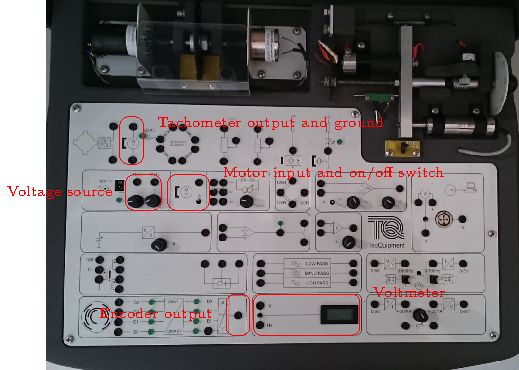
\includegraphics[width=0.7\linewidth]{figures/overview}
\caption{Relevant parts of the experimental device.}
\label{fig:equipment}
\end{center}
\end{figure}

\section*{Specifications}
\label{sec-2}

\begin{itemize}
\item Settling time ( \(\pm 5\%\) ) of 1 second
\item Overshoot of maximum 15\%
\end{itemize}

In order to determine the desired \textbf{continuous-time} poles of your closed-loop system, you may use the following relations for a second-order dominant system
\begin{description}
\item[{Settling time (5\%)}] \(t_s = \frac{3}{\zeta\omega_n}\)
\item[{Overshoot and damping ratio}] \[ \zeta = \sqrt{ \frac{(\ln \frac{PO}{100})^2}{\pi^2 + (\ln \frac{PO}{100})^2}}, \]
     where \(PO\) is the percent overshoot.
\end{description}

Observer poles (if needed) should be twice as fast as the closed-loop poles. Design a regular RST controller (not incremental).

\section*{Part 1 - Physical setup}
\label{sec-3}
\subsection*{Anti-aliasing filter}
\label{sec-3-1}
You will need to determine the sampling period \(h\) first, and then design a low-pass analog filter that will give good attenuation of signals above the Nyquist frequency. To keep things simple, it is suggested that you use a second order filter. Implement the filter in hardware, using op-amps, resistors and capacitors. 
\subsection*{Signal conditioner}
\label{sec-3-2}
Since the analog input channel of the Arduino expects a signal 0-5V, you need to design and implement a circuit that offsets and scale the output signal from the anti-aliasing filter in order to be in this range.

\subsection*{Motor driver}
\label{sec-3-3}
Since your microcontroller (typically) only provides analog output in the range 0-5V, you will need to design and implement a circuit that can deliver \textpm{} 5V.
\subsection*{Controller}
\label{sec-3-4}
The controller will run on your arduino. Send the control signal \(u(kh)\) and the measured angular position (encoder analog output) \(y(kh)\) to your computer so you can do system identification and plot results. 

\section*{Part 2 - System identification}
\label{sec-4}

\subsection*{Test setup}
\label{sec-4-1}
The idea is to send a suitable input signal to the DC motor and record the response. A pseudo-random binary sequence (PRBS) is often a good choice for the input signal. The amplitude should be sufficient to get good response from the motor. Since you are using a circuit to generate the input voltage to the DC motor, it makes sense to include this in the model of the plant, since it may have some non-neglectble dynamics. Thus, if your output signal from the arduino is a pwm analog signal in the range 0-5V, where 2.5V will give 0V to the DC motor, it makes sense to let your control signal be the deviation from 2.5V. Hence you can write the signal as 
\[ \bar{u}(t) = 2.5 + u(t) \]
where \(u(t)\) is your control signal.

The sampled output from the the plant \(y(kh)\) is the voltage from the encoder sensor, filtered through the anti-aliasing filter. Thus, also the anti-aliasing filter will be part of the identified plant model. 

\subsection*{Model selection and identification}
\label{sec-4-2}
In order to make the design of the controller simpler, assume a low-order model for the plant, for instance a second- or third-order model with delay (the delay is typically mostly due to the anti-aliasing filter). Do a long test (about one minute), so that you can divide the data set in modelling data and validation data. 

Make a simple arduino program that will perform the test on the system. Recording the input/output data can be done on a regular computer if you send the data over serial link. Use the system identification toolbox in matlab to identify your discrete-time model. Verify your model using the validation data. Include the plot of the model-output \(\hat{y}(kh)\) and the plant output \(y(kh)\) that shows how good the model is.  

\section*{Part 3 - Controller design and implementation}
\label{sec-5}
\subsection*{Determine the desired closed-loop poles}
\label{sec-5-1}
From the specifications, determine the desired continuous-time poles and transform these to the discrete-time. 

\subsection*{Design a 2-DoF controller}
\label{sec-5-2}
Assume a structure of the controller as given in figure \ref{fig:2dof}. The controller is given by 
\[ R(q)u = -S(q)y + T(q)u_c. \]
With the plant-model
\[ A(q)y = B(q)u\]
we get the following difference equation for the closed-loop system
\[ \big( A(q)R(q) + B(q)S(q) \big) y = B(q)T(q) u_c. \]
Determine the order (as low as possible) of the controller polynomials $R(q)$ and $S(q)$ and solve the diophantine equation 
\[ A(q)R(q) + B(q)S(q)  = Ac(q) \]
for $R$ and $S$. 

\begin{figure}
\begin{center}
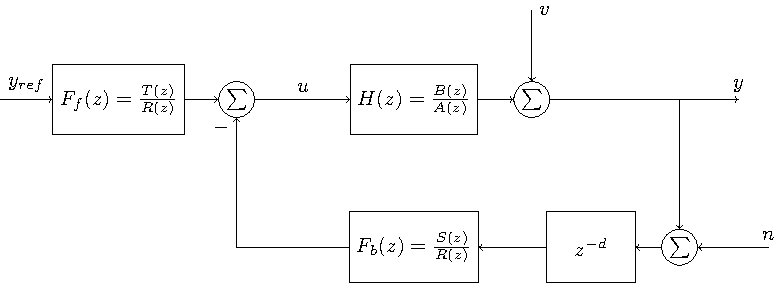
\includegraphics[width=0.6\linewidth]{./2dof-block-explicit}
\caption{Closed-loop system with two-degree-of-freedom controller}
\label{fig:2dof}
\end{center}
\end{figure}

\subsection*{Deadzone compensation}
\label{sec-5-3}
The DC-motor has  deadzone, meaning that the motor will not move unless the voltage is above a certain value. Determine this deadzone by connecting the reference voltage to the motor as seen in figure \ref{fig:deadzone-experiment}. You can read off the voltage from the LCD-display.
\begin{figure}
\begin{center}
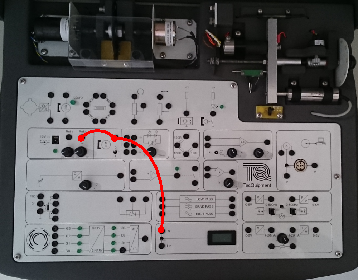
\includegraphics[width=0.6\linewidth]{figures/deadzone-setup}
\caption{Connections for checking the deadzone of the DC motor.}
\label{fig:deadzone-experiment}
\end{center}
\end{figure}

The deadzone can be compensated by inverting the deadzone function. In practice this means  adding (or subtracting) to the control signal, the offset corresponding to the deadzone. Your controller algorithm should do this compensation just before writing the value to the analog output of the arduino. The code should do something like this
\begin{verbatim}
const float deadzonePos = 0.8; # Or what you determine
const float deadzoneNeg = 0.9;

float y = current_position(); # Read the angular position signal y
float uc = current_command(); # Read the command input

float u = next_control_signal(y, uc); # Calculate the control signal u

if (u>0) {
   u = u + deadzonePos;
else {
   u = u - deadzoneNeg;
}

write_control_signal(u); # Write control signal to output channel
\end{verbatim}

\subsection*{Implementation and tests}
\label{sec-5-4}
Implement your RST controller on the microcontroller. Run some step responses on the closed-loop system. Plot the results from these, and verify that the closed-loop system satisfies the specifications.

\section*{Report}
\label{sec-6}
Document your work in a laboratory report. It should be possibly to repeat your work based on the report, so include code and brief, but complete descriptions. Include graphs to illustrate your results. The report should have the following sections
\begin{enumerate}
\item Introduction
\item Circuit design and physical setup
\item Plant model and identification
\item Controller design
\item Implementation and results
\item Conclusion
\item Appendix: Your lab notes.
\end{enumerate}
% Emacs 24.5.1 (Org mode 8.2.10)
\end{document}